\section{Commit}
\subsection{Erster Commit}
Um den aktuellen Status zu protokollieren wird der Befehl \inline{git commit} genutzt. Dabei werden alle Änderungen an allen Dateien protokolliert, die sich im Status \qq{staged} befinden.

Ist eine Datei neu (war vorher also im Status \qq{untracked}) wird dabei eine Kopie der Datei in \inline{.git} abgelegt. Ist die Datei nur verändert wurden (war vorher somit im Status \qq{modified}) wird nur die Information über die Änderung gespeichert.

Ein Commit besteht aus mehreren Teilen: 
\begin{itemize}
	\item Ein tree Objekt, welches den Hash des Aktuellen Zustands des Projektes angibt
	\item Ein \qq{parent} Objekt, der Hash des \qq{parent} Commits
	\item Name und Email-Adresse des Autors
	\item Name und Email-Adresse des Committers
	\item Head der Commit-Message (CM)
\end{itemize}
CM sollten möglichst einheitlich und übersichtlich gestaltet werden. Für Programmcodes gibt \cite{conv-Commit} eine gute Zusammenfassung, wie CM strukturiert werden können\footnote{In dem Beispiel git zu diesem Bericht wird davon jedoch nicht vollständig Gebrauch gemacht, da es für Latex Dokumente nicht geeignet ist.}.

Wenn der Befehl \inline{git commit} ohne Optionen ausgeführt wird öffnet sich automatisch der Standard-Editor, welcher über \inline{git config --local core.editor} definiert wurde. In diesem befindet sich eine auskommentierte Übersicht des Commits. Darunter muss eine CM eingefügt werden. Wird der Editor geschlossen ohne, dass neue Zeilen hinzugefügt wurden bricht der Commit ab.
\begin{figure}[!h]
        \centering
        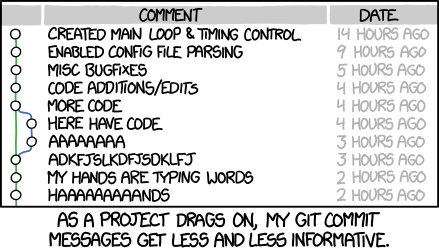
\includegraphics[width=0.5\textwidth]{Bilder/git_commit.png}
        \caption{Eine Commit-Baum-Darstellung von XKCD \cite{Munroe}. Die CM starten oben mit den ersten Commits sehr vorbildlich. Nach einigen Commits ist zu sehen, dass die CM keine Informationen über den Commit Inhalt mehr haben. Dies ist ein häufiges Problem, wenn zu selten committed wird kann es schnell passieren, dass nicht mehr klar ist, was sich seit dem letzten Commit alles geändert hat. Dadurch werden CM schnell schwer zu schreiben und vernachlässigt.}
        \label{fig:Commit-XKCD}
\end{figure}

In Abb. \ref{fig:Commit-XKCD} ist ein sogenannter Commit-Baum dargestellt. In einem Commit-Baum werden alle existierenden Commits aufgelistet und \qq{parent} und \qq{child} Commit miteinander verbunden. Neben jedem Commit wird der jeweilige Commit-Header angezeigt. Solch ein Commit-Baum sollte eine gute Übersicht über den Verlauf der Entwicklung eines Programms geben. Daher müssen Commit-Header möglichst eindeutig und einheitlich verfasst werden.

In Abb. \ref{fig:Commit-XKCD} sieht man jedoch, dass es zunehmend schwerer werden kann zu einem Commit eine gute Beschreibung zu finden. Wenn z.B. viele Änderungen in einem Commit zusammengefasst werden kann es schwer sein einen geeigneten Commit-Header zu finden.

Nachdem ein Commit erfolgt ist befinden sich alle Dateien, die vorher im \qq{staging} Status waren im \qq{unmodified} Status (siehe Abb. \ref{fig:lifecycle}). 
\begin{mplisting}
$ git status
On branch master
nothing to commit, working tree clean
\end{mplisting}
%
\subsection{Gitignore}
In den meisten Projekten existieren Dateien, welche nicht innerhalb der Versionskontrolle verfolgt werden sollen. Im Fall dieses Latex Dokumentes z.B. sind dies die Auxilliar-Dateien, welche beim compilieren der PDF entstehen. Um solche Dateien nicht immer als \qq{untracked} angezeigt zu bekommen können sie explizit aus dem Repository ausgeschlossen werden. Dafür nutzt man eine Datei namens \inline{.gitignore}. Diese muss im root Ordner des Repositories erstellt werden. Alle innerhalb dieser Datei aufgelisteten Ordner und Dateien werden nicht von Git beachtet.

Nach dem Kompilieren des Projektes sieht Git alle Auxiliar-Dateien als \qq{untracked}:
\begin{mplisting}
$ git status
On branch master
Untracked files:
	(use "git add <file>..." to include in what will be committed)
		main.aux
		main.bbl
		main.bcf
		main.blg
		main.log
		main.out
		main.pdf
		main.run.xml
		main.synctex.gz
		main.toc
nothing added to commit but untracked files present (use "git add" to track)

\end{mplisting}
fügt man diese Dateien jedoch einer \inline{.gitignore} hinzu:
\begin{mplisting}
$ echo "main.aux
	main.bbl
	main.bcf
	main.blg
	main.log
	main.out
	main.pdf
	main.run.xml
	main.synctex.gz
	main.toc" >> .gitignore
$ git status
On branch master
Untracked files:
(use "git add <file>..." to include in what will be committed)
.gitignore

nothing added to commit but untracked files present (use "git add" to track)
\end{mplisting}
ignoriert Git alle aufgelisteten Dateien und findet nur noch die neue Datei \inline{.gitignore}.

\subsection{Zurücksetzen auf vorhergehenden Commit}
In diesem Abschnitt wird kurz erklärt, wie man das Projekt auf einen bestimmten Commit zurücksetzen kann.

Um ein Projekt zurücksetzen zu können, muss der Ziel-Commit identifiziert werden können. Dafür ist jedem Commit ein eindeutiger Hash-Wert zugewiesen. Eine liste dieser Hashs\footnote{Git nutzt für die Hashs SHA1 Checksummen von den Commit-Objekten. Weitere Informationen dazu können in \cite{ProGit} gefunden werden.} kann mit \inline{git log} angezeigt werden:
\begin{mplisting}
$ git log
commit b7c5da73f9fce4176f37c5af0e929107da168adb (HEAD -> master)
Author: Till Hanke <till.hanke@student.uni-halle.de>
Date:   Wed Jul 29 16:20:47 2020 +0200

    style: change listings style
    
    basicstyle of listings is set to small.

commit b0002ceccd3566f61c3b33772ebd0ac286f9013f
Author: Till Hanke <till.hanke@student.uni-halle.de>
Date:   Wed Jul 29 16:15:20 2020 +0200

    add: gitignore with all aux files listed

commit 016591903c23f9a66e76a699139cc93918ea17a6
Author: Till Hanke <till.hanke@student.uni-halle.de>
Date:   Wed Jul 29 16:13:19 2020 +0200

    intermediate: commit to clear git status
\end{mplisting}
Hier is ein kurzer Auszug des Logs zu sehen. Der oberste Commit ist der aktuelle \qq{HEAD}, d.h. der letzte Commit. Erkennbar ist es daran, dass hinter dem Hash des Commits \inline{HEAD -> master} steht. \inline{master} ist ein Verweis auf den aktuellen Branch (was das bedeutet wird in Kapitel \ref{sec:branch} erklärt).

Unter dem Hash des Commits steht der Autor, welcher den Commit veröffentlicht hat und dessen Email-Adresse.
Außerdem ist der Zeitstempel des Commits angegeben. Zuletzt und eingerückt wird der Header der CM ausgegeben.

Um eine abgekürzte Version des Logs zu sehen sind folgende Optionen hilfreich:
\begin{mplisting}
$ git log --pretty=format:"%h %s" 
b7c5da7 style: change listings style
b0002ce add: gitignore with all aux files listed
0165919 intermediate: commit to clear git status
3421046 add: subsection about gitignore
8608c08 add: final part of commit section
bcdca21 remove: mplisting styles removed
\end{mplisting}

Wenn der korrekte Hash gefunden wurde (z.B. \inline{016591903}) kann der Master Branch darauf zurückgesetzt werden indem man \inline{git reset} nutzt. Dabei muss nicht der gesamte Hash angegeben werden, sondern nur so viel, dass der Commit eindeutig identifiziert ist.
\begin{mplisting}
$ git reset --hard 3421046
HEAD is now at 3421046 add: subsection about gitignore
$ git log --pretty=format:"%h %s" 
3421046 add: subsection about gitignore
8608c08 add: final part of commit section
bcdca21 remove: mplisting styles removed
\end{mplisting}
In dem Log ist zu erkennen, dass die letzten drei Commits nun weg sind. Jedoch sind auch diese Commits dadurch nicht verloren gegangen, sondern können mit demselben Befehl wiederhergestellt werden. Dafür wird nur der Hash des Commits benötigt, der wiederhergestellt werden soll. Diese Commits können im Referenz-Log (\inline{git reflog}) gefunden werden:
\begin{mplisting}
$ git reflog
3421046 (HEAD -> master) HEAD@{0}: reset: moving to 3421046
b7c5da7 HEAD@{1}: commit: style: change listings style
b0002ce HEAD@{2}: commit: add: gitignore with all aux files listed
0165919 HEAD@{3}: commit: intermediate: commit to clear git status
3421046 (HEAD -> master) HEAD@{4}: commit: add: subsection about gitignore
8608c08 HEAD@{5}: reset: moving to 8608c08eddc0fb893ccd88887889900b29aa6122
b8f2753 HEAD@{6}: commit: add: subsection about gitignore
8608c08 HEAD@{7}: commit: add: final part of commit section
bcdca21 HEAD@{8}: commit: remove: mplisting styles removed
\end{mplisting}
In diesem Log sind alle Aktionen des lokalen Repositories aufgelistet. Es ist zu sehen, dass der Commit, auf den der \inline{master} Branch gerade verweist zweimal vorkommt (Zeile 2 und Zeile 6). Zwischen diesen beiden Einträgen sind die vorhergehenden Commits zu sehen.






